\section{DSP}
The \emph{OMAP3530} GPP contains a \emph{TMS320} DSP (\emph{DSP})\cite{gpp-refman}. This
core is optimised for using multiple calculation channels simultaneously: it is
a \emph{VLIW} (Very Long Instruction Word) processor that can utilise eight
functional units at the same time. More specifically, we can use six ALUs and
two multipliers per instruction. Another interesting feature is that each
multiplier can perform two 16 x 16-bit multiplications as well\cite{dsp-refman}, giving us
potentially four multiplications in parallel.

The GPP unit is responsible for starting up the DSP core, giving it an executable to run
and afterwards detaching the core. Furthermore, the requirements specified
that the matrices to multiply are generated on the GPP core (which is
of course not a bad idea because the GPP is way more flexible: it can easily
be changed to read the matrices from a file or standard input, and we can
offload a part of the work to the GPP itself and also the \emph{NEON} as we
will discuss later as well).

\subsection{Communication}
This however brings us to one complication: the matrices have to be moved to
the DSP core, while the (partial) end result has to be sent back to the GPP.
Our first goal is thus to set up communications and send matrices back and forth
between the two cores.

\begin{figure}[h]
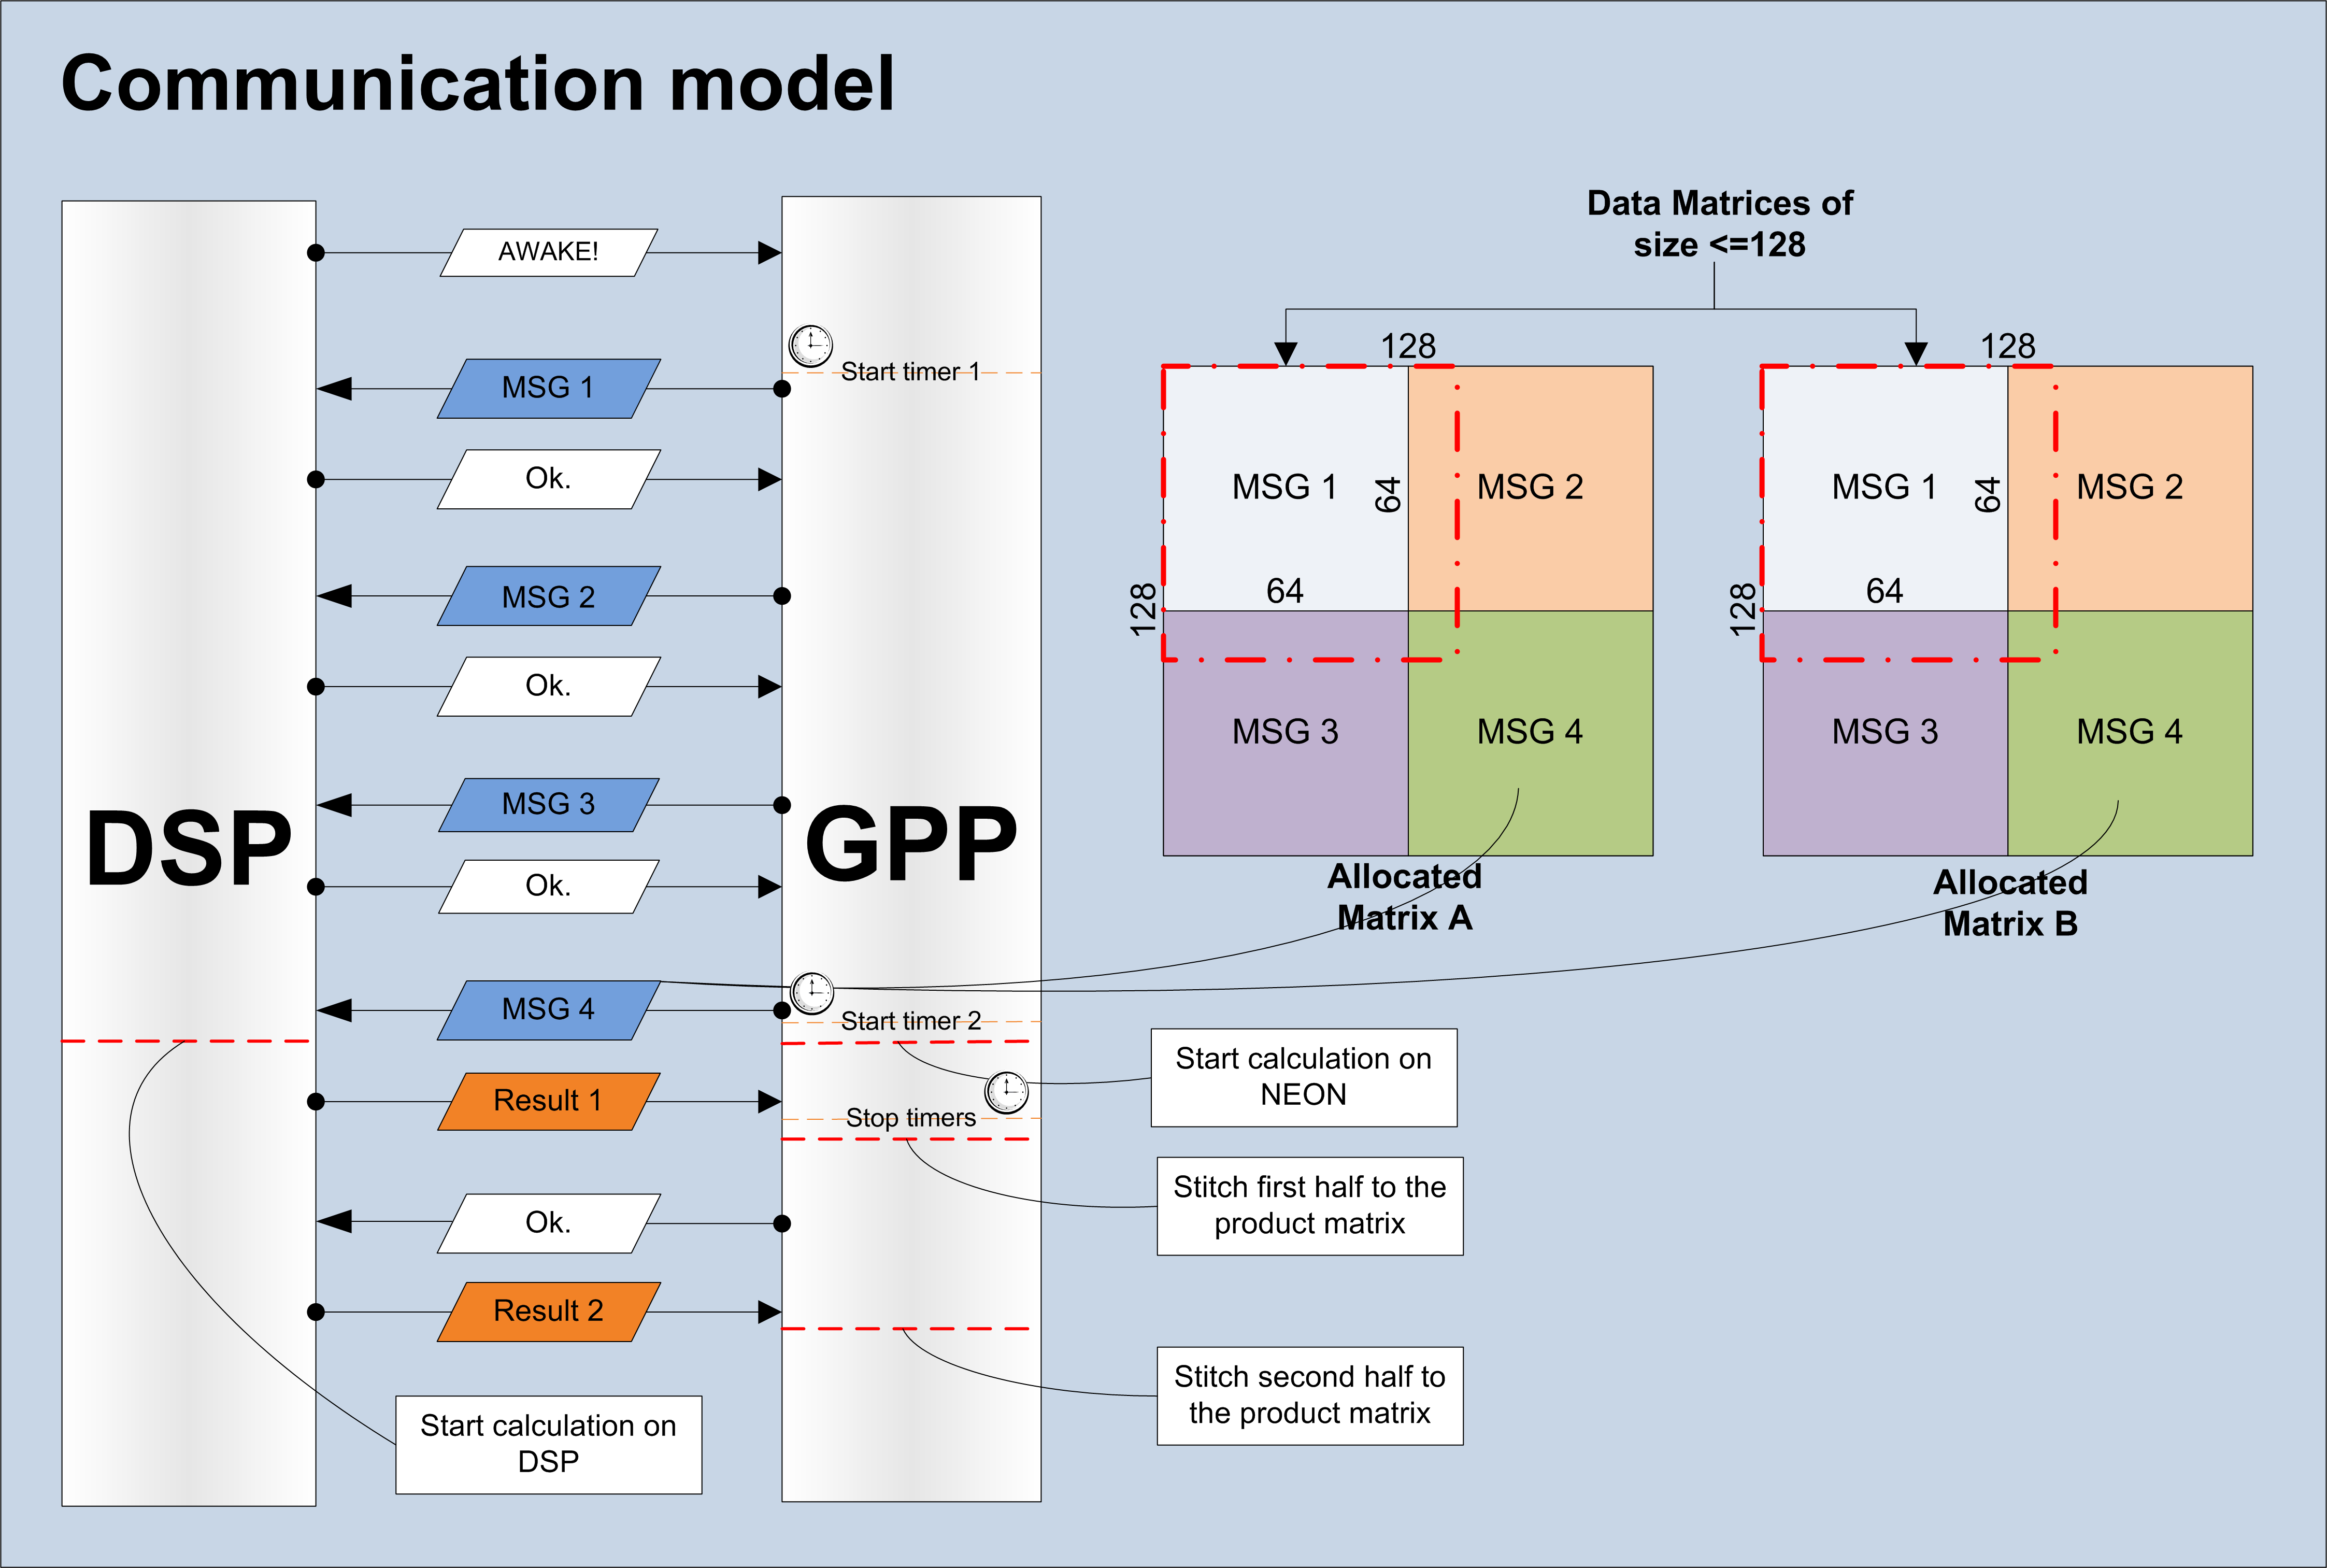
\includegraphics[width=\textwidth]{images/gpp_dsp_com}
\caption{Describing the communication process between the cores over time}
\label{fig:gpp_dsp_com}
\end{figure}

Unfortunately the communication API is slightly verbose and hard to handle.
For example, the sender has to allocate memory for a message, send it and the
receiver has the possibility to send it back, or free the message. If we opted
for the latter and re-allocate every message we would always crash the DSP core.
The former option would mean that if we wanted to send more than one message
directly from the GPP, the DSP would have to send the entire message back first.
We however observed that the communication overhead is negligible, so we
decided to always re-use the same message. The general communication time-line
is described in figure~\ref{fig:gpp_dsp_com}. One observation in this time-line
is that we send data six times. The reason why will be discussed in the next
section.

\subsubsection{Message Format}
We used the existing reference communication implementation and it's message
structure, but we extended it with our own matrices and an extra field that
indicates how big the resulting matrix should be. One thing we had to do
was determine the maximum matrix size we could assign, such that it would fit
in one message. This message would be stored inside a section of
\emph{APP\_BUFFER\_SIZE} large, thus our message structure has to fit in there.
This buffer was $16768$ bytes on our system.
Removing the (negiglable) overhead of $279$ bytes our payload limit is $16489$ bytes.

The source matrices are 16 bit, but the result should be at least 32 bits.
To accommodate for both
situations in the same control message structure while optimally using our
message in a uniform way, we opted to use a \emph{union} structure so we
can either send two 16 bit matrices or one 32 bit matrix at a time. The
structure is given in figure~\ref{code:control_msg}.

Because we have to send up to $128*128*2*2=65536$ (2 matrices of 16 bits)
bytes from the GPP to the DSP, we need at least four messages considering
our bandwidth limit of $16489$ bytes. Thus we send the source in four messages,
each containing a quarter of both matrices. The DSP only calculates a half of
the result matrix, making two messages sufficient: this results in six
communication steps.

\begin{figure}[h]
\begin{lstlisting}[language=C]
struct mat2x16 {
	int16_t mat1[SIZE][SIZE];
	int16_t mat2[SIZE][SIZE];
};

struct mat32 {
	int32_t mat1[SIZE][SIZE];
};

typedef union {
	struct mat2x16 m16;
	struct mat32 m32;
} mat_t;

#define ARG_SIZE 256
typedef struct ControlMsg
{
    MSGQ_MsgHeader header;	// 20 bytes
    Uint16 command;				// 2 bytes
    Char arg1[ARG_SIZE];		// 256 bytes
    Uint8 size;					// 1 byte
    mat_t mat;						// 4 * SIZE * SIZE bytes
} ControlMsg;
\end{lstlisting}
\caption{The message structure we used}
\label{code:control_msg}
\end{figure}


\subsubsection{Communication Details}
This section describes the communication model in more detail.

Figure~\ref{fig:gpp_dsp_com} shows how packets are communicated between the two cores. Initially the GPP gets an AWAKE message from the DSP indicating that communication is established and further actions may begin.
Then we initiate the transfer of data (multiplicand and multiplier matrices) to DSP. Since the packet is fixed in size and not dynamic (as described in the section above) and the actual matrix size is <=128 we have decided to fill in the allocated matrix of size 128 with the given size matrix as shown on the right hand side of the figure in order not to over complicate the process.
So in the next four iterations the GPP sends a quarter of every matrix to the DSP along with the size of the data matrices since the DSP must know what is being multiplied from the received matrices of size 128. As soon as the GPP sends the fourth message (MSG 4) it immediately begins to calculate the partial product. Similarly as soon as the DSP receives the fourth (final) message it begins doing its partial product calculation and initiates MSGQ\_put() which places the first half of the partial product onto the communication channel (Result 1) followed by the next massage (Result 2). On the other hand, the GPP initiates a MSGQ\_get() action as soon as it is done with its calculations to receive Result 1 and 2 from DSP and stitch the product together.
In order to examine the results (that are presented later in this report) we put timers in the appropriate places. The first timer is put immediately after the generation of multiplicand and multiplier matricies and before MSG 1 is being transmitted such that to take into account the communication overhead and measure the entire execution time.
The second timer is placed immediately after MSG 4 is send. The second timer gives us the upperbound on max(ARM, DSP) execution times while neglecting the communication time as much as possible. Both timers are stopped as soon as the calculations are done and the first packet from the DSP (Result 1) is received. In the analysis we would be focusing more on the first timer.
Also note that there are many different possibilities to place the timers however we figured timer 1 is optimal as it incorporates most of delays, and provides good insight when doing analysis.
